\documentclass[border=8pt]{standalone}
\usepackage{amsmath}
\usepackage{tikz}
\usetikzlibrary{arrows.meta,positioning,calc,decorations.pathreplacing}
\begin{document}
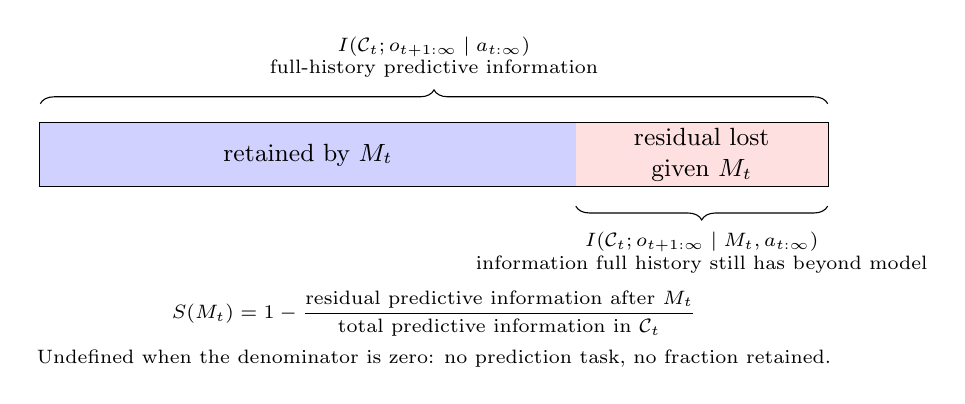
\begin{tikzpicture}[
  note/.style={align=center, font=\scriptsize},
  label/.style={align=center, font=\small}
]

\draw[thick] (0,0) rectangle (10,0.8);
\fill[blue!18] (0,0) rectangle (6.8,0.8);
\fill[red!12] (6.8,0) rectangle (10,0.8);

\node[label] at (3.4,0.4) {retained by $M_t$};
\node[label] at (8.4,0.4) {residual lost\\given $M_t$};

\draw[decorate, decoration={brace, amplitude=5pt}] (0,1.05) -- node[above=6pt, note] {$I(\mathcal C_t; o_{t+1:\infty}\mid a_{t:\infty})$\\full-history predictive information} (10,1.05);

\draw[decorate, decoration={brace, mirror, amplitude=5pt}] (6.8,-0.25) -- node[below=6pt, note] {$I(\mathcal C_t; o_{t+1:\infty}\mid M_t,a_{t:\infty})$\\information full history still has beyond model} (10,-0.25);

\node[note, below=1.2cm] at (5,0) {$S(M_t)=1-\dfrac{\text{residual predictive information after }M_t}{\text{total predictive information in }\mathcal C_t}$};
\node[note, below=1.95cm] at (5,0) {Undefined when the denominator is zero: no prediction task, no fraction retained.};

\end{tikzpicture}
\end{document}
